\chapter{Muons in ATLAS}
  
\textit{I really need to find a quote for this chapter}
\vspace{5mm}
\begin{flushright}
--- Miha Zgubi\v{c}
\end{flushright}

\thispagestyle{empty}
\newpage
The ATLAS detector, described in the previous chapter, is a monument
to the engineers and physicists who designed and built it. However,
in order to turn its raw output of nearly one hundred million readout
channels per event to physics knowledge, it requires an intermediate step:
the reconstruction of physics objects.

Muons, the central physics object in this thesis, are reconstructed
by combining the information from the tracker and the muon spectrometer.
In order to be able to do precision studies the Monte Carlo (MC)
simulation of the detector response needs to be calibrated to match
the response in the real detector. In particular, the transverse momentum of
muons needs to be calibrated to the resolution obtained in the real
detector. Similarly, the reconstruction, track-to-vertex-association (TTVA),
and isolation efficiencies need to be calibrated to match those in 
recorded data. These calibrations are obtained through measurements
and carry associated uncertainties.

This chapter describes the first novel contributions from the author.
The first is an improved method of background subtraction in the isolation
efficiency measurements, which significantly reduces the systematic
uncertainty for muons with $\pt < 15$ \GeV. The second is an attempt
to improve muon momentum resolution.

\section{Reconstruction}

Tracks in the inner detector (ID) are reconstructed indiscriminately for
all charged particles. First, raw data from the detectors is converted
into space-points which form the basis of tracking. The main track finding
algorithm proceeds inside-out by finding the seeds in the silicon layers.
The seeds are then combined into roads and the extension to the TRT layer
is probed to add hits in the outermost layer. The final collection of hits
is fit to obtain the track parameters \cite{ATLAS-CONF-2010-072, Cornelissen:1020106}.
Tracks with at least $\pt > 400$ \MeV~and some other requirements, found
in Ref. \cite{ATL-PHYS-PUB-2015-026} are then used to find the primary
vertices. The reconstruction of primary vertices proceeds by first finding
the vertices and then fitting them \cite{Aaboud:2016rmg}. Finally, tracks
are associated with vertices which allows the computation of $d_0$, the
transverse impact parameter, which quantifies the shortest distance
between the track and the beam-line, and $z_0$, the longitudinal impact
parameter, which quantifies the difference between the $z$ coordinate
of the associated primary vertex, and the $z$ coordinate of the point
where $d_0$ is computed.

The reconstruction of tracks in the muon spectrometer (MS) proceeds by
first finding track segments in the MDT chambers using a Hough transform
\cite{ILLINGWORTH198887}, and then reconstructing them by fitting a
straight line to the associated hits. The segments are combined to
form MS tracks starting from the middle layer and finding compatible
segments in the inner and outer layers of the spectrometer. At least two
segments are needed to form a track, apart from the transition region
in which a single high quality segment can be used to build a track.
Finally, a global $\chi^2$ fit of the track is performed and the track
accepted if it satisfies the quality criteria. Otherwise, hits with 
high contribution to the $\chi^2$ value are removed and the track re-fit.
Hits can also be added to the track if they are consistent with the
track and the track is re-fit if these candidates are found \cite{Aad:2016jkr}.

Finally, the information from subdetectors is combined to form muon
candidates. Depending on which subdetectors are used for building the
candidate, four muon types are defined:
\begin{itemize}
\item Combined (CB) muons are reconstructed from a pair of tracks
in the ID and the MS. A global re-fit is performed using hits from 
both subdetectors with the flexibility to add or remove hits in the
MS to improve the fit quality. Most muons are reconstructed by the
outside-in approach extrapolating the MS tracks to the ID, but the
inside-out reconstruction is also used as the complementary approach 
\cite{Aad:2016jkr}.
\item Segment-tagged (ST) muons are formed by combining the ID track
with a single segment in the MDT or CSC chambers and were designed
to recover muon reconstruction efficiency for low $\pt$ muons which
only cross a single layer of the MS or cross the regions where
MS has poor acceptance \cite{Aad:2016jkr}.
\item Calorimeter-tagged (CT) muons match an ID track with a 
calorimeter deposit consistent with a minimum-ionising particle.
This type recovers the muon reconstruction efficiency in the regions
not covered by the MS, for example in the $|\eta|<0.1$, where cabling
and services to the ID are located, and where the support structure
is located. As a consequence of using the calorimeter this type has
the lowest purity \cite{Aad:2016jkr}.
\item Extrapolated (ME) muons are built from tracks in the MS that
are loosely compatible with originating from the interaction point.
This type is used to recover the reconstruction efficiency in the 
forward region $2.5 < |\eta| < 2.7$ not covered by the ID \cite{Aad:2016jkr}.
\end{itemize}
Finally, overlaps between different muons are resolved by order of
precedence starting with CB muons, followed by ST muons, and
finally the CT muons. ME ambiguities are resolved by analysing the
track fit quality and the number of hits.
The requirements on the number of hits and holes
\footnote{A \textit{hole} is an active sensor traversed by the
track that contains no hits. It also falls between two hits assigned to the track.}
in the ID and MS detectors are also used to guarantee a robust
measurement of $\pt$ \cite{Aad:2016jkr}.

In addition to that, a number of quality requirements must be
satisfied to differentiate between muons originating from the
interaction point (prompt muons) and the muons coming from the
decay of light hadrons. To this end the following variables are
defined for CB muons:
\begin{itemize}
\item normalised $\chi^2$ of the combined track fit.
\item $\rho' = \frac{|\pt^{\text{ID}} - \pt^{\text{MS}}|}{\pt^{\text{CB}}}$,
where the superscript denotes whether the $\pt$ refers to the
ID or MS muon candidate, or the CB muon.
\item $q/p$ significance $ = \frac{\left|\left(\frac{q}{p}\right)_\text{ID}
- \left(\frac{q}{p}\right)_\text{MS}\right|}
{\sqrt{\sigma^2_\text{ID} + \sigma^2_\text{MS}}}$,
where the $\left(\frac{q}{p}\right)$ is the measurement of the ratio of
the charge and the momentum, $\sigma$ are the uncertainties on
the corresponding quantities, and the subscript refers to whether
the measurement comes from the ID or the MS muon candidate.
\end{itemize}

Four overlapping muon identification selections, namely Loose, Medium, Tight,
and High-$\pt$, are supported by the muon performance group to 
serve different physics analyses and unify the evaluation of
systematic uncertainties arising from the selection requirements.
Tight muons maximise the purity of muons at the cost of some
identification efficiency and use only CB muons with additional
requirements on the track quality. Medium muons include CB and ME
muon types and are the default selection that minimises the systematic
uncertainties. Loose muons are designed to maximise the selection
efficiency and include all four muon types, with the CT and ST types
restricted to the $|\eta| < 0.1$ \cite{Aad:2016jkr}.

The fraction of prompt muons that are reconstructed and identified
is called reconstruction efficiency, and is in general different
in data and MC simulation. Efficiencies for Loose, Medium, and Tight
selections are shown in Figure \ref{fig:muon:reco_eff} for data and
MC simulation as a function of muon pseudorapidity. In the analysis,
MC simulation is corrected to data by applying weights, known as
scale factors, to account for the differences in efficiencies between
data and MC simulation. The scale factors (SF) are defined as
\begin{equation}
\text{SF} = \frac{\epsilon_\text{Data}}{\epsilon_\text{MC}},
\end{equation}
where SF is the scale factor, and $\epsilon$ is some efficiency,
as measured in data or MC simulation. The measurement of the
efficiencies, scale factors, and the associated
uncertainties is described in detail in Ref. \cite{Aad:2016jkr}.

\begin{figure}[h]
  \centering
  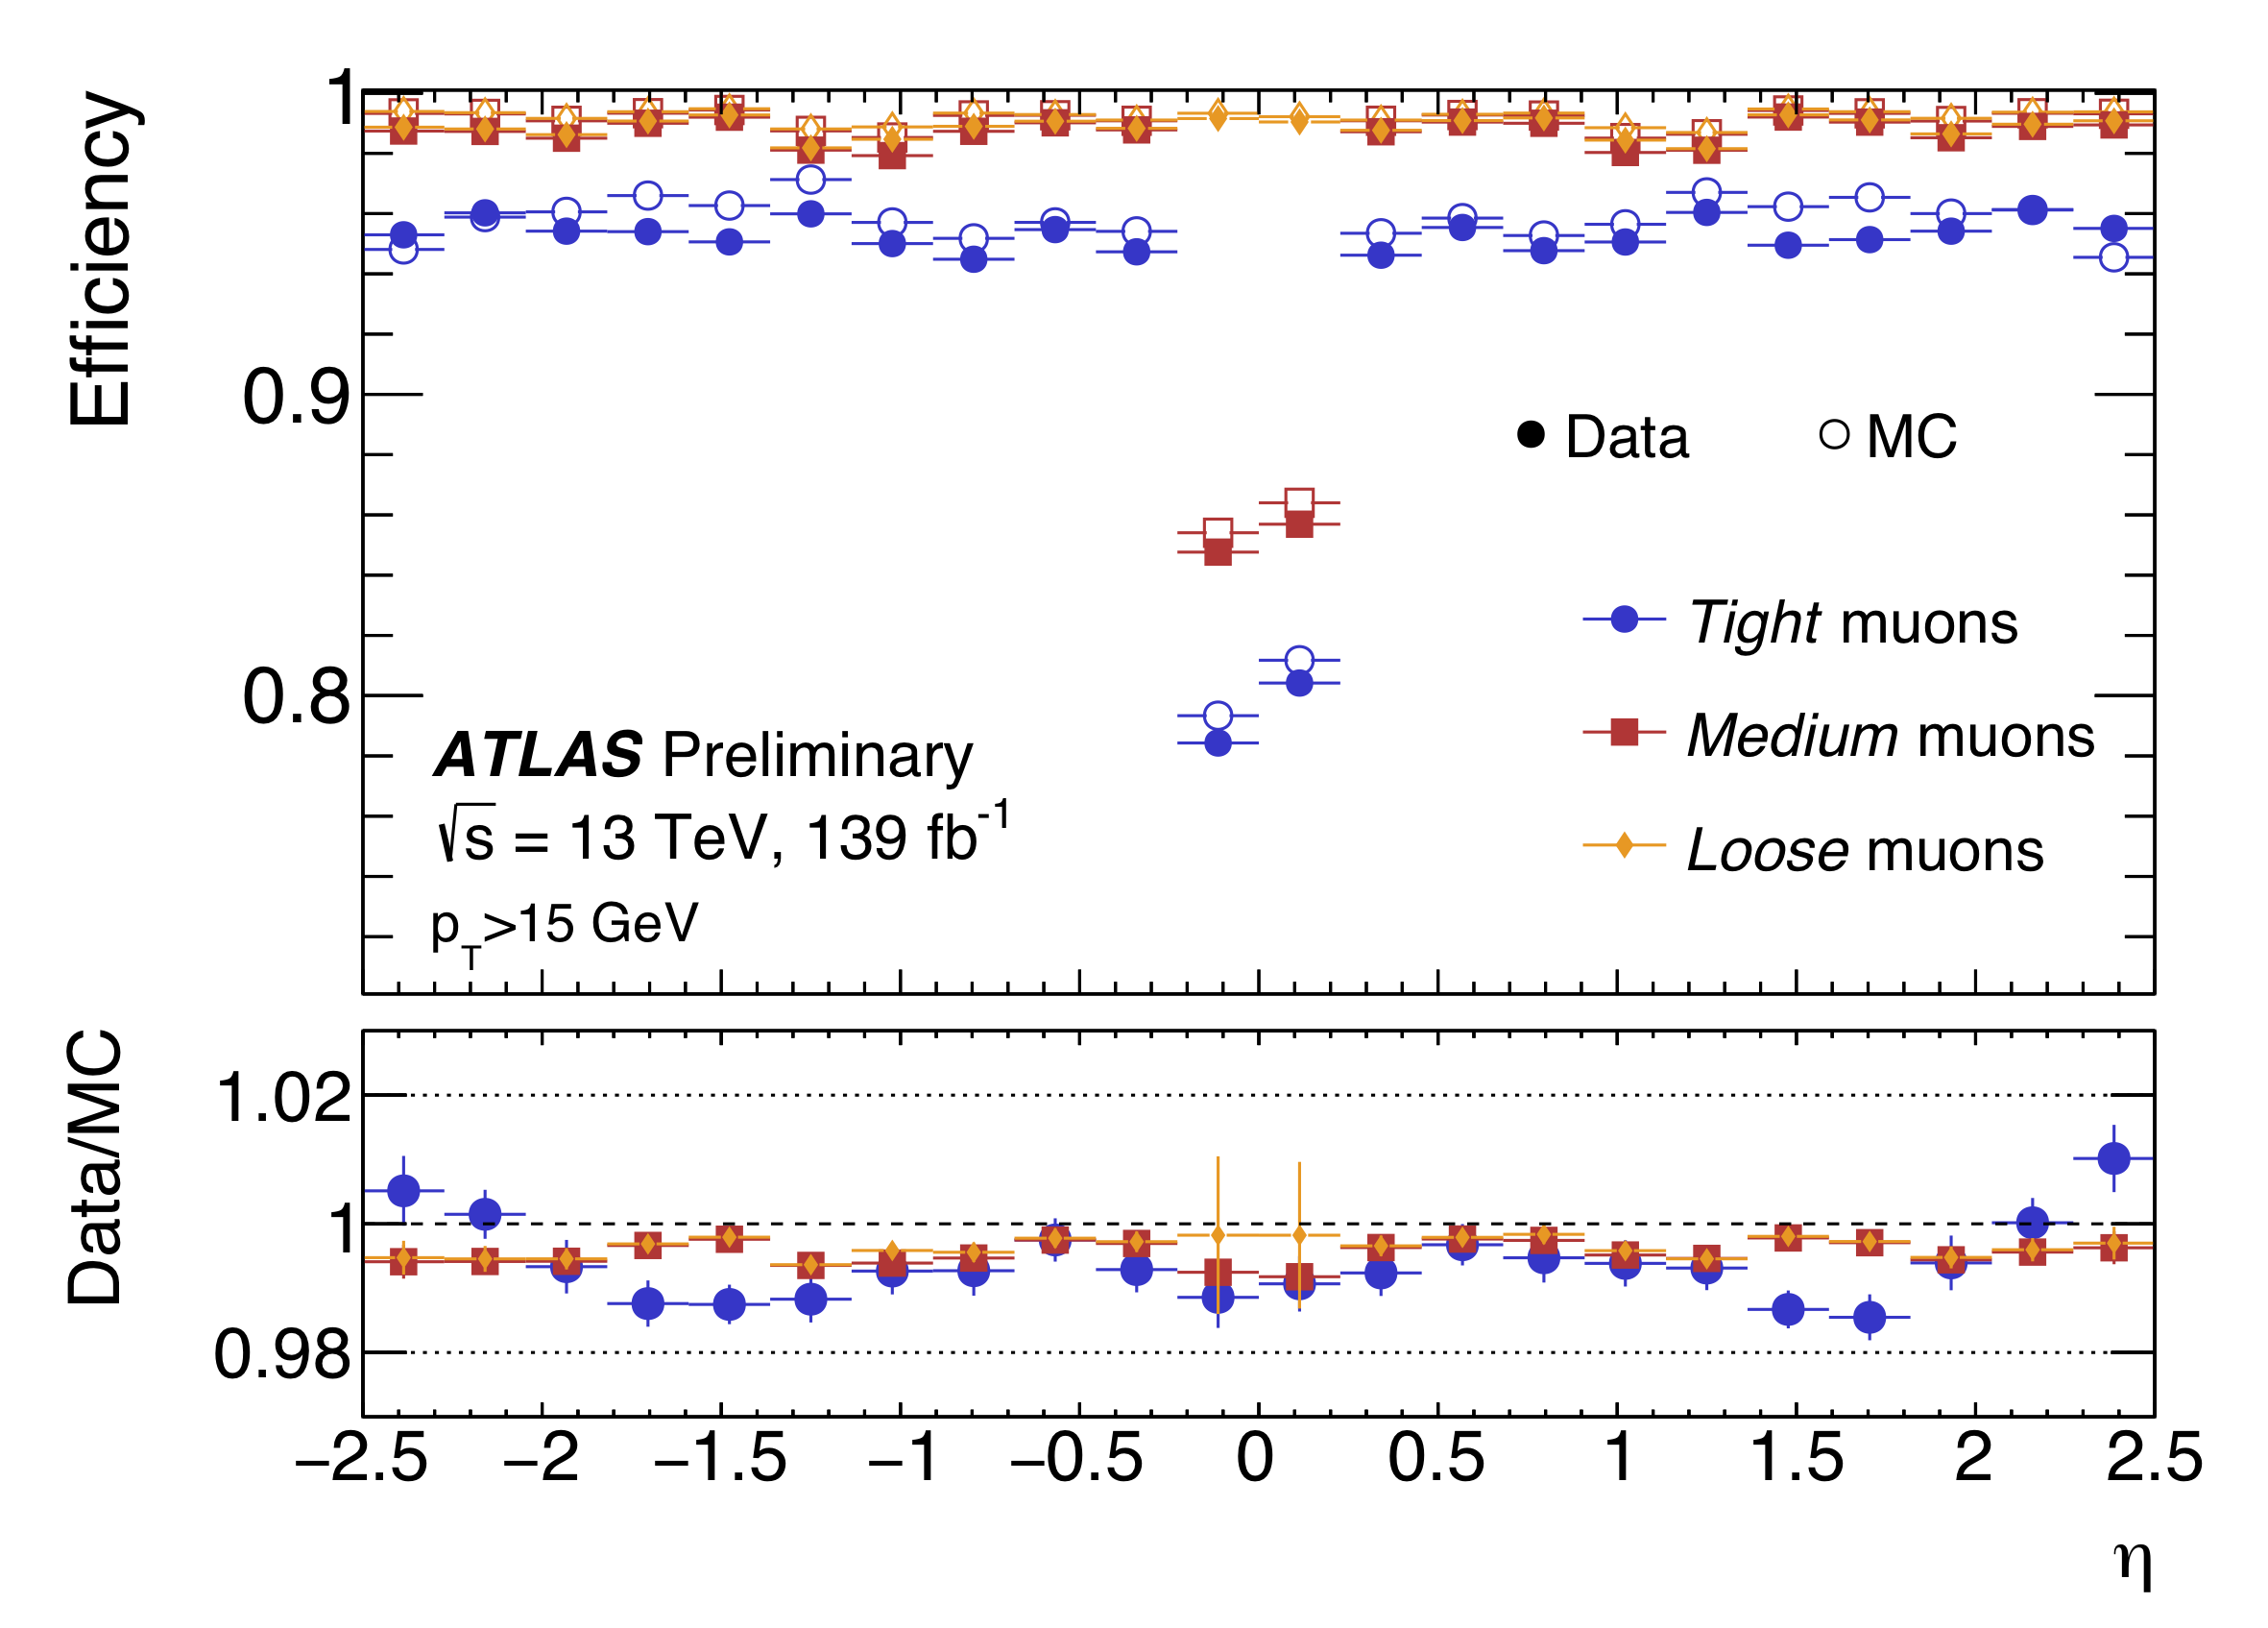
\includegraphics[width=0.8\textwidth]{figures/muons/reco_eff}
  \caption[Muon reconstruction efficiency.]{Muon reconstruction
  efficiency measurement for the Loose (yellow diamonds), Medium
  (red squares), and Tight (blue circles) selections in data
  (filled markers) and MC simulation (empty markers) as a function
  of muon pseudorapidity with $\pt > 15~\GeV$. The measurement
  uses $\zmumu$ events in full Run 2 dataset of 139 $\ifb$
  at $\sqrt{s}=13~\TeV$. Error bars represent a quadratic sum of
  statistical and systematic uncertainties. From Ref. \cite{Junggeburth:2685295}.}
  \label{fig:muon:reco_eff}
\end{figure}

\section{Momentum calibration}

The response of the ATLAS detector is accurately modelled by the
MC simulation. However, additional momentum calibration of MC simulation
is needed to achieve per mille level precision in muon momentum scale
and percent level precision in momentum resolution \cite{Aad:2016jkr}.

The corrections are applied separately to ID and MS tracks and 
have a dependence on the $\eta$ and $\phi$ of the muon track. The
corrected momentum
\begin{equation}
\pt^\text{Cor} = \frac{\pt + \sum_{n=0}^1 s_n(\eta, \phi) \cdot \pt^n}
{1 + \sum_{m=0}^2 \Delta r_m (\eta, \phi) \cdot \pt^{m-1} \cdot g_m},
\label{eq:muon:calibration}
\end{equation}
where $s_n(\eta, \phi)$ are the scale corrections, and
$\Delta r_m (\eta, \phi)$ are the resolution corrections,
and $g_m$ is a random variate from a normal distribution with zero mean
and variance of 1, 
can be computed from the uncorrected transverse momentum in simulation,
$\pt$, once the values of $s_n$ and $\Delta r_m$ are known \cite{Aad:2016jkr}. The
denominator in Eq. \ref{eq:muon:calibration} assumes that the relative
transverse momentum resolution can be parametrised as
\begin{equation}
\frac{\sigma(\pt)}{\pt} = \frac{r_0}{\pt} \oplus r_1 \oplus r_2 \cdot \pt
\end{equation}
where the $r_0$ term accounts for the fluctuations of the energy loss, the
$r_1$ term for multiple scattering, and the $r_2$ term for the
resolution in the measurement of the sagitta due to intrinsic hit resolution
and misalignment of the MS \cite{Aad:2016jkr}.

The corrected momentum of CB muons is then determined by combining the
corrected momenta of ID and MS muons
\begin{equation}
\pt^\text{CB, Cor} = f \cdot \pt^\text{ID, Cor} + (1-f) \cdot \pt^\text{MS, Cor},
\end{equation}
with the weight $f$ derived for each muon individually from the equivalent
equation with uncorrected momenta, thus assuming the relative contributions
of the two subdetectors are unchanged by the momentum corrections \cite{Aad:2016jkr}.

The determination of $s_n$ and $\Delta r_m$ constants proceeds by an
iterative fitting procedure described in detail in Ref. \cite{Aad:2016jkr}.
It extracts the constants by binned maximum likelihood fits of the
invariant mass spectra of $Z\rightarrow\mu\mu$ and $J/\psi\rightarrow\mu\mu$.
The validation of the calibration using CB muons in $Z\rightarrow\mu\mu$
events is shown in Figure \ref{fig:muon:calibration} as a function of the
pseudorapidity of the leading muon. 

\begin{figure}[h!]
  \centering
  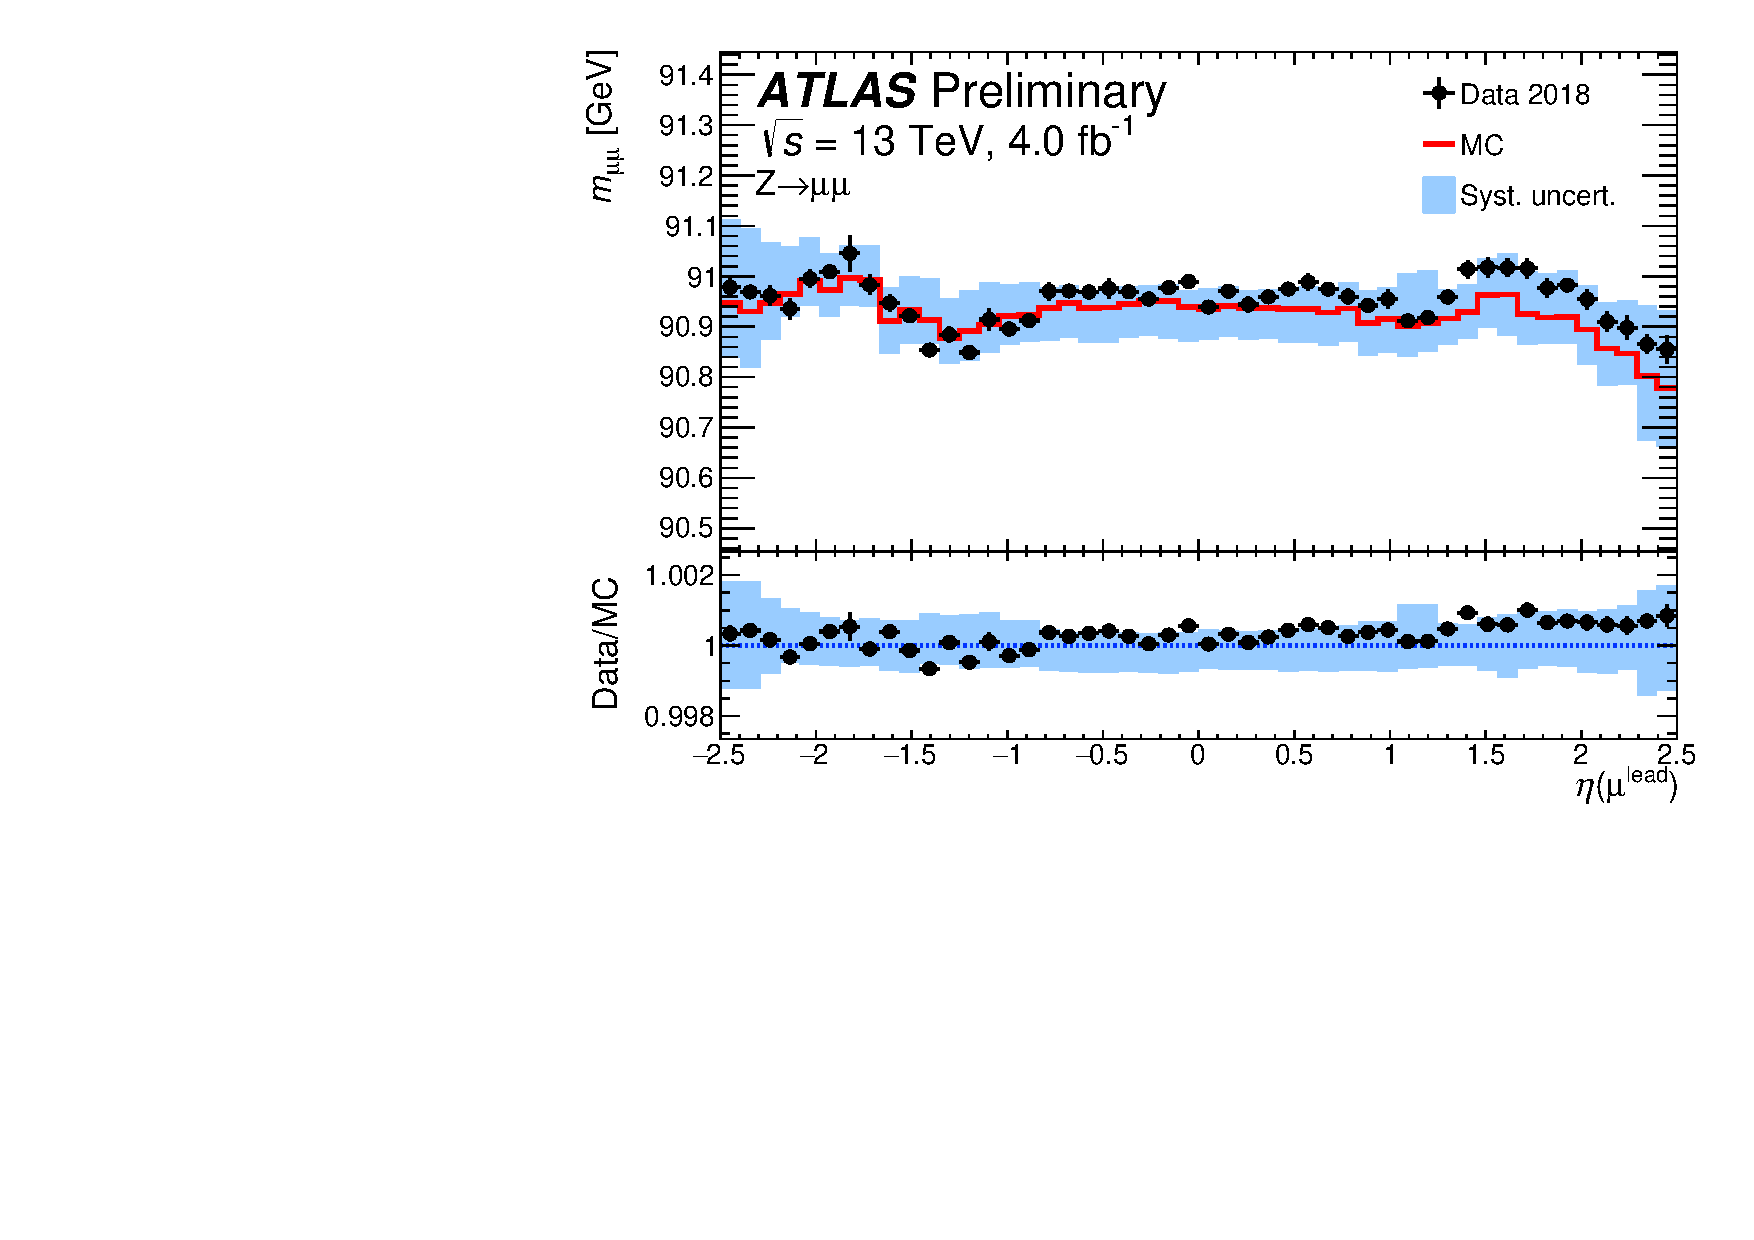
\includegraphics[width=0.8\textwidth]{figures/muons/scale} \
  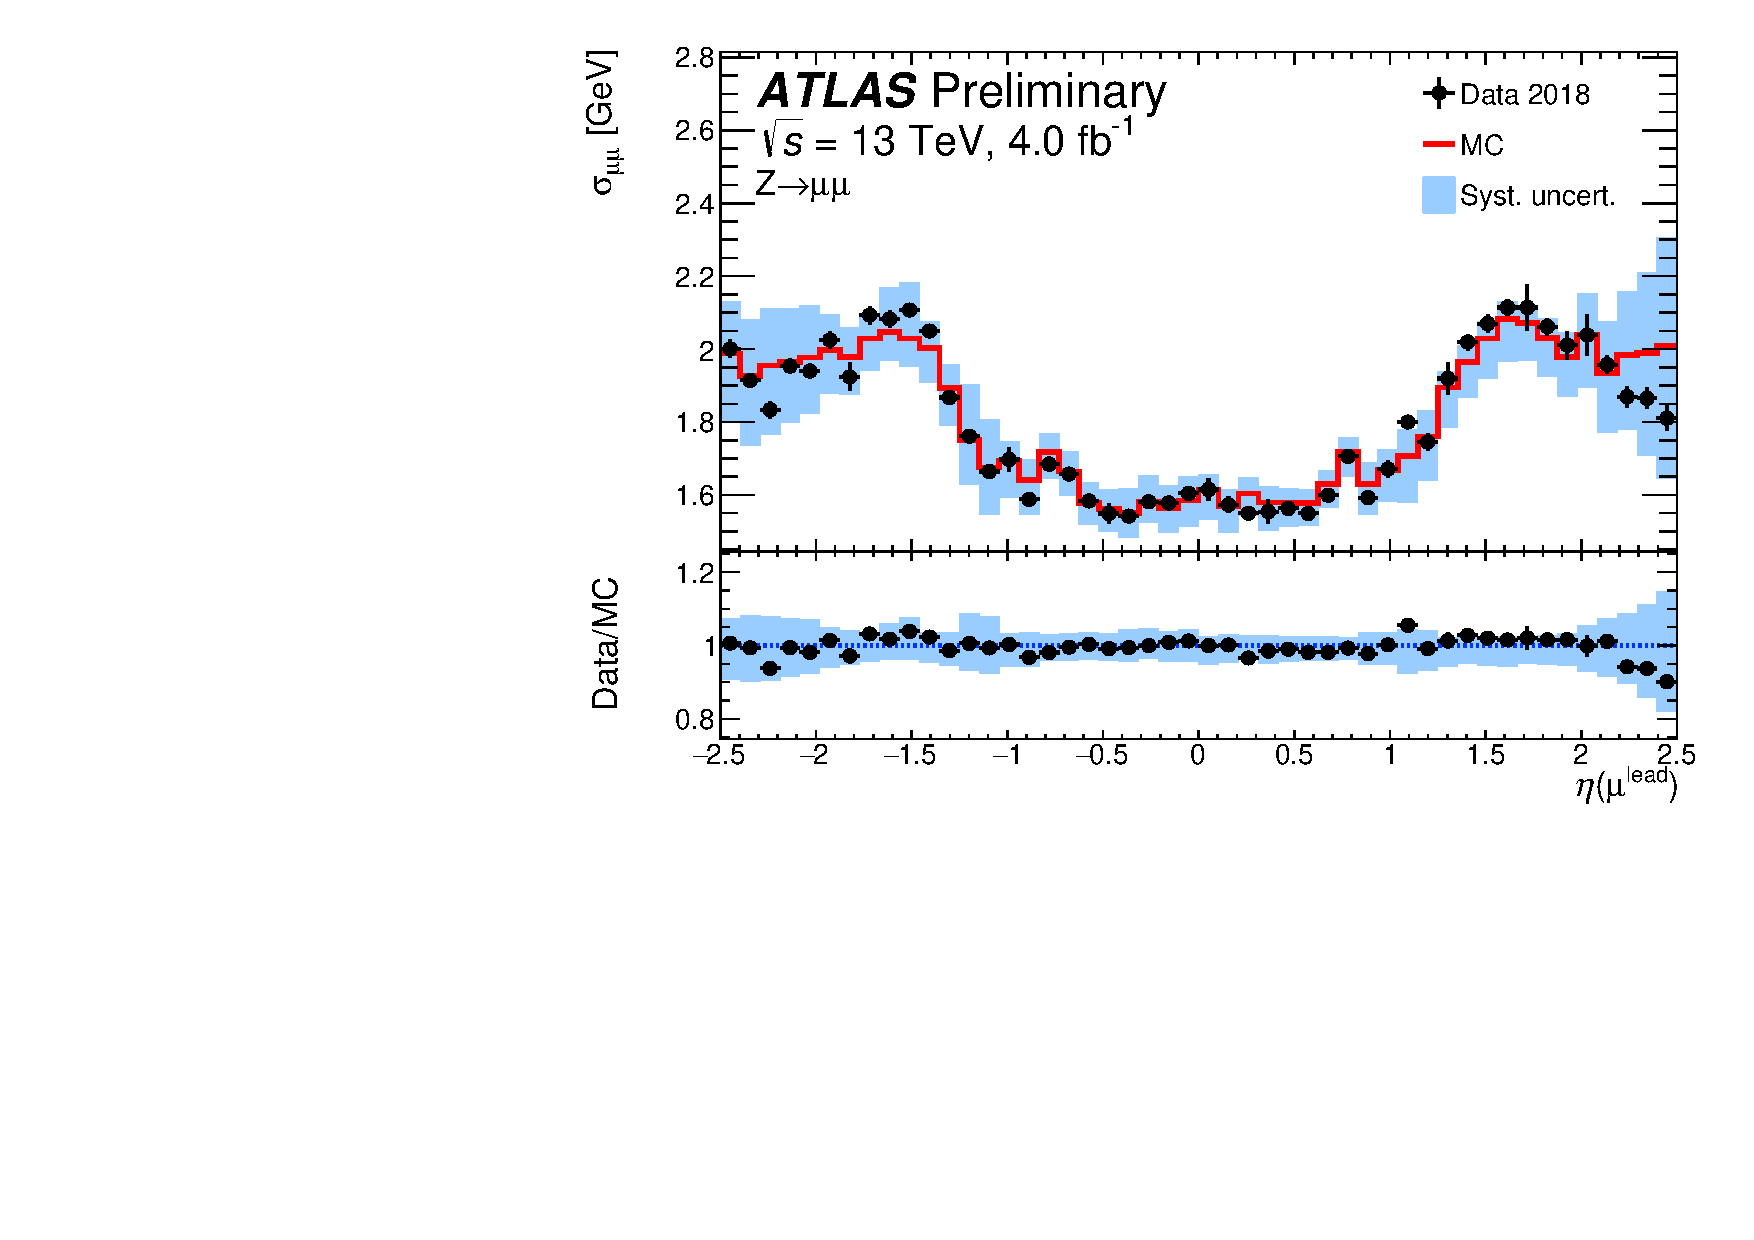
\includegraphics[width=0.8\textwidth]{figures/muons/reso}
  \caption[Muon calibration validation.]{Muon calibrations
  validation compares the scale (top) and resolution (bottom)
  of $Z\rightarrow\mu\mu$ events using CB muons in part of
  2018 data (black circles) to the corrected MC simulation
  (red line). The systematic uncertainty on the corrected MC
  simulation is shown as blue bands. The bottom panel in each
  figure shows the ratio between the data and MC simulation.
  From Ref. \cite{Barone:2320120}}
  \label{fig:muon:calibration}
\end{figure}

\section{Isolation}

Prompt muons, produced at the interaction point or from the decay of heavy
bosons, often need to be distinguished from muons coming from a secondary
vertex as a result of the decay of a $\tau$ lepton, heavy quarks, or
hadrons. Other processes can also fake a muon signature in the detector,
for example a jet punching through the hadron calorimeter in the muon
spectrometer could be reconstructed as a muon. The key to identification
of non-fake prompt muons is that they are produced in isolation from
other particles, unlike fake or non-prompt muons which are usually
surrounded by a jet of other particles. Two sets of variables, one based
on the tracker information and the other on calorimeter information, are
used to identify prompt muons.

Track-based isolation variable, $\pt^{\text{varcone}, R}$, is defined
as the scalar sum of $\pt$ of non-muon tracks inside the cone of radius
$\Delta R = \min(R, 10~\GeV/\pt^\mu)$, where $R = \sqrt{\Delta \eta^2 +
\Delta \phi^2}$ and $\pt^\mu$ is the transverse momentum of the muon.
The tracks used in the sum have $\pt > 1~\GeV$,
$|\eta| < 2.5$, longitudinal impact parameter $< 3~\mm$, and satisfy a
Loose track quality. The cone size is chosen to vary with $\pt^\mu$
to follow the collimation of tracks in highly boosted systems \cite{Aad:2016jkr}.

Calorimeter-based isolation variable relies on the notion of a topological
cluster, built by seeding the cluster with a calorimeter cell with
signal-to-noise (S/N) greater than four, adding the neighbouring cells with
S/N $ > 2$, and finally adding the surrounding cells \cite{Aad:2011he}. The
variable $E_\text{T}^\text{topocone20}$ is defined as the sum of
the transverse energy of topological clusters in a cone of size $\Delta
R = 0.2$, after subtracting for the energy deposited by the muon itself
and the estimate of the energy coming from \pileup~related effects. The
\pileup~contributions are estimated using jet area technique \cite{CACCIARI2008119}
and are corrected on event-by-event basis \cite{Aad:2016jkr}.

Isolation selections are defined as cuts on these variables. Various
selections have been supported in the past few years, to target the needs
of different analyses and to adapt to higher \pileup~conditions. The 
selections differ in signal efficiency and backgorund rejection
throughout the $\pt$ regime. For each of the isolation selections a
measurement of efficiencies in data and MC simulation is performed, as
well as the evaluation of scale factors, which vary as a function
of muon $\pt$. The measurement of the efficiencies is performed on
$Z\rightarrow\mu\mu$ events in data and MC simulation using the
tag-and-probe method \cite{Aad:2016jkr}.

Tag-and-probe selects events with a pair of muons with invariant mass
within 10 GeV of the $Z$ boson mass, where the tag muon is required to
have triggered the event, and the probe muon is used for the efficiency
measurements. More precisely, the tag muon is required to satisfy
$\pt > 24~\GeV$, pass Loose isolation selection, and must be trigger
matched to the muon firing the trigger. Both tag and probe muons are
required to be CB muons, passing the Medium quality requirements,
and pass requirements on transverse and longitudinal impact parameters
or their significances $d_0/\sigma_{d_0} < 3.0$, $|z_0| < 10~\mm$ and
$|z_0 \sin{\theta}| < 0.5~\mm$. They are also required to be well
separated $R_{\mu,\mu} > 0.3$ from each other, and the probe should
be separated from jets $R_{j,\mu} > 0.4$.

The MC simulation contains a pure sample of $Z\rightarrow\mu\mu$ events,
but the recorded data consists of an unknown mixed stream of underlying
processes, both the $Z\rightarrow\mu\mu$ decays as well events with fake
or non-prompt muons, collectively referred to as background. In order
to measure the efficiency of prompt muons, the background must be
subtracted in the efficiency measurement in data. The old method of
background subtraction relied on the assumption that the number of
background events in data is the same in the same charge
(SC) as in the opposite charge (OC) phase space:
\begin{equation}
\epsilon_{\zmumu} =
\frac{N_\text{match}^\text{OC} - T \cdot N_\text{match}^\text{SC}}
     {N_\text{probe}^\text{OC} - T \cdot N_\text{probe}^\text{SC}},
\end{equation}
where $T$ is the transfer factor, $N_\text{probe}$ is the number of
probe muons and $N_\text{match}$ is the number of probe muons passing
the isolation selection in either SC or OC phase space, as indicated by
the superscript. The leading systematic uncertainty at low muon $\pt$
comes from the background subtraction, namely the assumption $T=1$.
Additional systematic uncertainties on the scale factor
measurement are computed by varying the selection requirements and
adding individual unceratinties in quadrature, and adding a fixed
uncertainty due to variation in $\eta$ as the scale factors are
provided only as a function of $\pt$. The systematic variations are
summarised in Table \ref{tab:muon:systs} below.
\begin{table}[h]
\centering
\caption{Systematic uncertainties in the measurement of the isolation
selection scale factors.}
\label{tab:muon:systs}
\begin{tabular}{c c}
\toprule
Description & Variation \\
\midrule
Background estimation         & $T=0.5, T=2.0$ \\
Dependence on $\eta$          & Flat 0.2\% uncertainty \\
$m_{\mu\mu}$ window           & $m_Z \pm 5, 20~\GeV$ \\ 
Probe muon quality            & Loose, Tight \\
Tag muon isolation            & Every other isolation selection \\ 
Probe muon to jet separation  & $\Delta R_{j, \mu} > 0.3, 0.5$ \\
Probe to tag muon separation  & $\Delta R_{\mu, \mu} > 0.2, 0.5$ \\
\bottomrule
\end{tabular}
\end{table}
The scale factors are evaluated as a function of probe muon $\pt$,
with uncertainties compute in each bin separately. At low $\pt$
($< 15~\GeV$), the leading uncertainty is the background subtraction,
which prompted the development of a new background subtraction
method, described in the next section.

\section{Isolation efficiency background subtraction}

The core idea of the novel background subtraction method is to
reduce the assumption that the number of SC events is the same as
the number of OC events, to the assumption that the shape of the
invariant mass spectrum for background events is the same in the
SC and OC events. The SC region is used to determine the shape
of the background events, while the normalisation is determined
from the template fit to OC data.

Efficiency measured in data is a sum of efficiencies of the
components, weighted by the component fractions
\begin{equation}
\epsilon_\text{measured} =
\text{f}_{\zmumu}   \cdot \epsilon_{\zmumu} +
\text{f}_\text{EWK} \cdot \epsilon_\text{EWK}
\text{f}_\text{QCD} \cdot \epsilon_\text{QCD},
\end{equation}
where $f$ represents the fraction of the component, and $\epsilon$
the efficiency of the component. Subscript QCD refers to the
background component due to muons in jets, and EWK refers to the
background from electroweak processes\footnote{Consists of
$W^\pm\rightarrow\mu^\pm \nu$, $Z\rightarrow \tau\tau$,
$WW\rightarrow \ell \nu \ell \nu$, $WZ\rightarrow \ell \nu \ell \ell$,
$WZ\rightarrow qq \ell \ell$, $ZZ\rightarrow\ell\ell\ell\ell$,
$ZZ\rightarrow\nu\nu\ell\ell$, $ZZ\rightarrow qq\ell\ell$,
$t\bar t$ MC samples generated with \textsc{Powheg}+\textsc{Pythia}8.}.
The efficiency of $\zmumu$ events in data can therefore be expressed as
\begin{equation}
\epsilon_{\zmumu} = \frac
{\epsilon_\text{measured} - \text{f}_\text{EWK} \cdot \epsilon_\text{EWK} - \text{f}_\text{QCD} \cdot \epsilon_\text{QCD}}
{1 - \text{f}_\text{EWK} - \text{f}_\text{QCD}},
\end{equation}
where $\text{f}_{\zmumu} = 1 - \text{f}_\text{EWK} - \text{f}_\text{QCD}$
was used. The efficiency $\epsilon_\text{EWK}$ is measured in MC,
while the efficiency $\epsilon_\text{QCD}$ is measured in SC data.

The fractions $\text{f}_\text{EWK}$ and $\text{f}_\text{QCD}$ are
determined via a template fit to the OC data, shown in Figure
\ref{fig:muon:fit}, in each of the $\pt^\text{probe}$ bins.
The shapes of the templates are allowed to vary in the fit within
statistical uncertainties.
\begin{figure}[h!]
  \centering
  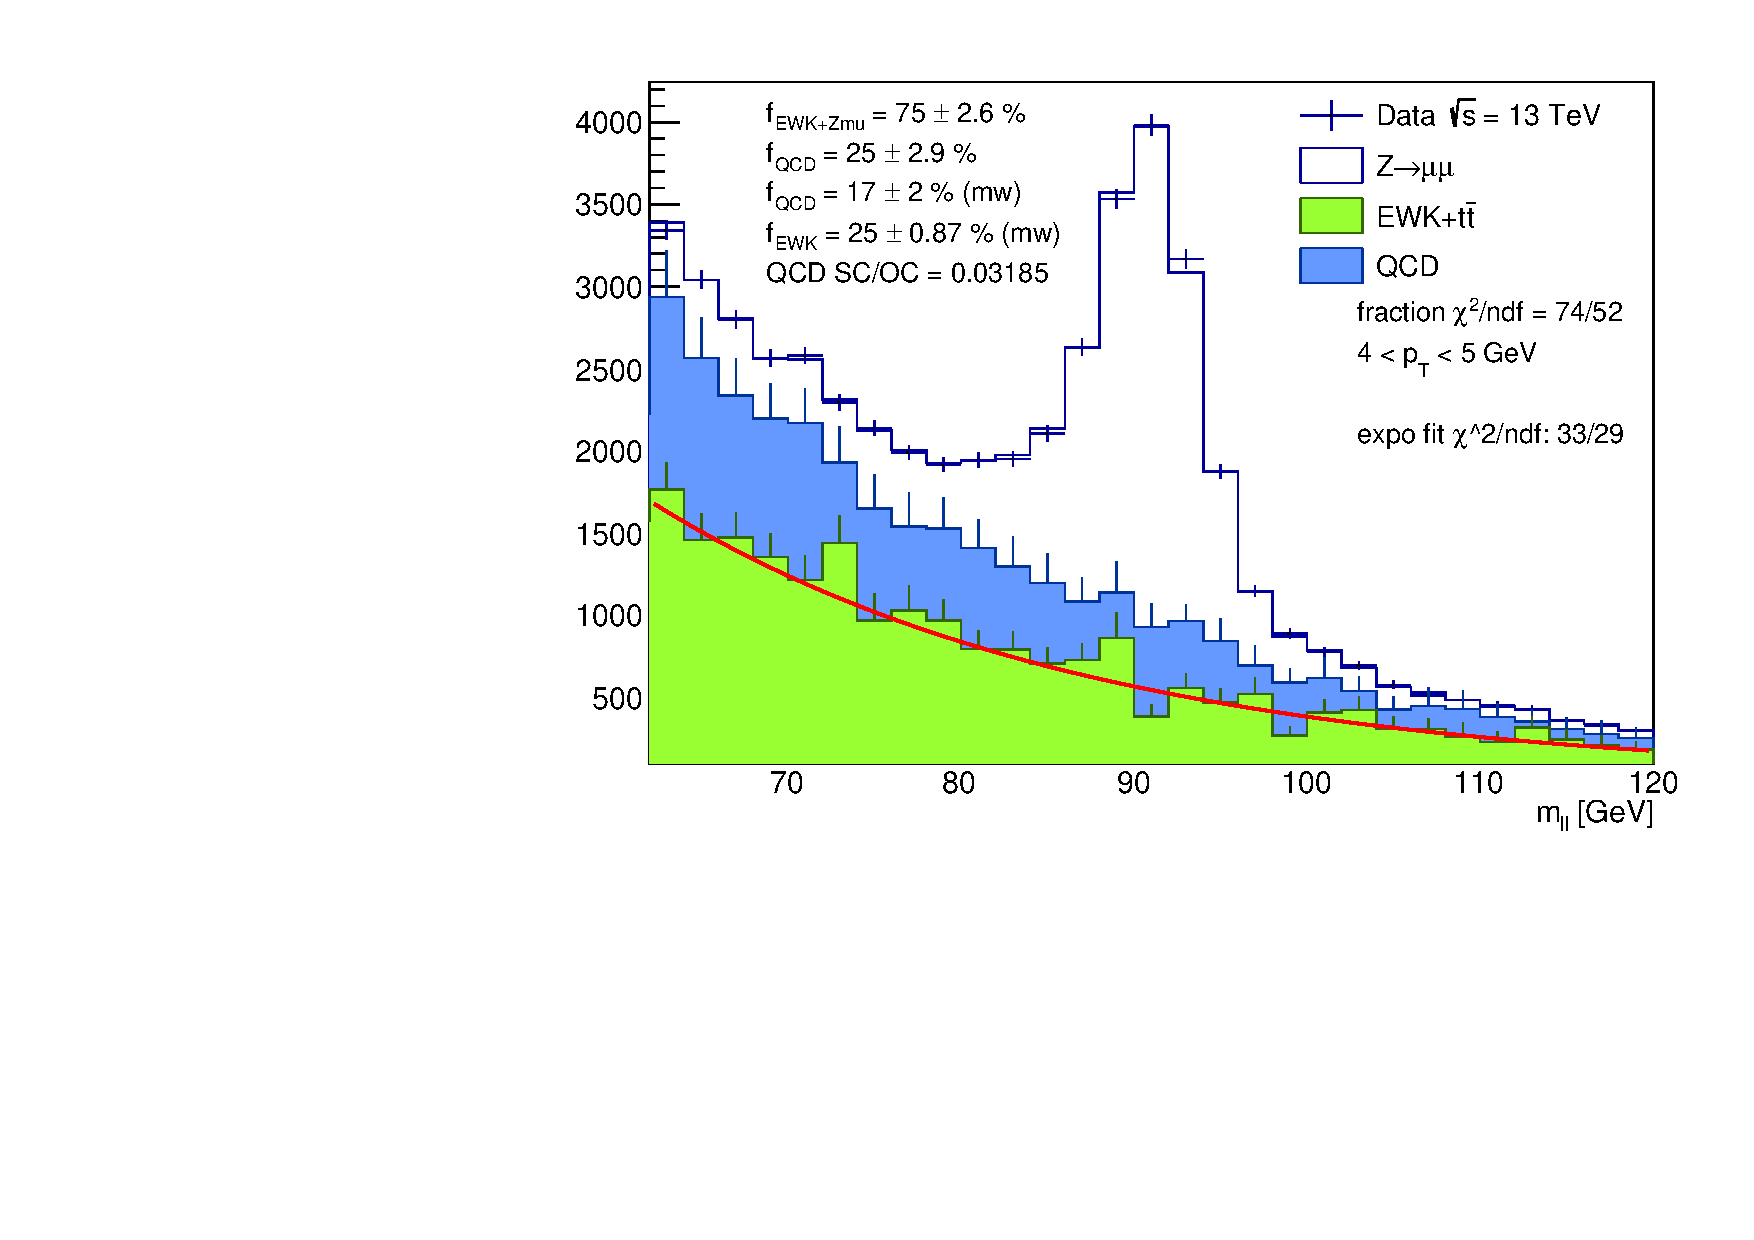
\includegraphics[width=0.8\textwidth]{figures/muons/fit}
  \caption[Muon isolation background subtraction fit.]{Muon isolation
  background subtraction template fit in OC data to determine the
  $\text{f}_\text{EWK}$ and $\text{f}_\text{QCD}$ fractions in the
  $4 < \pt^\text{probe} < 5~\GeV$ bin.
  Data is shown as blue points, QCD template, taken from SC data, is
  shown in blue. The other template is determine from MC and is a
  combination of the $\zmumu$ events, shown in white, and the EWK
  processes, shown in green. Error bars show statistical
  uncertainties. A maximum likelihood fit with the exponential
  function to the EWK component is shown in red. The reduced $\chi^2$
  values are shown on the figure for both the template fit and the
  subsequent exponential function fit. Furthermore, fraction values
  are shown both for the full invariant mass range, over which the
  fit is performed, and in the $\pm 10~\GeV$ mass window (mw) around
  the $Z$ peak.}
  \label{fig:muon:fit}
\end{figure}
While the fit is performed over a wide invariant mass range ($\pm30~\GeV$)
around the $Z$ peak, the fractions need to be determined in a narrower
mass range in which the efficiency measurement is made ($\pm10~\GeV$).
This is done by integrating the fitted templates in the desired range,
using linear interpolation where necessary. For the EWK template, in
order to decrease the statistical fluctuations, an exponential fit
to the template is integrated instead. When varying the mass range
of the measurement, as shown in Table \ref{tab:muon:systs}, the fractions
are recomputed in the adjusted range.

The current method no longer assumes that the normalisation of background
events is the same in SC and OC data. Instead, the assumption is reduced
to the shape of the background to be the same, with normalisation 
determined via the fit. In order to estimate the associated systematic
uncertainty the scale factors are re-computed using different QCD templates.
Recall, the nominal template is taken from the SC data, where the number of
genuine $\zmumu$ events is negligible. Similarly, two other templates are
constructed in the $\zmumu$ depleted regions, where the requirement on the
impact parameter significance ($|d_0/\sigma_{d_0}|$) is inverted in both
the SC and OC data. Region definitions are shown in Table \ref{tab:muon:reg}.
\begin{table}[h]
\centering
\caption{Region definitions from which the QCD template shape is taken
for the isolation background subtraction fit.}
\label{tab:muon:reg}
\begin{tabular}{c c c c c}
\toprule
Region   & Charge & $\pt^\text{probe}$ range & $|d_0/\sigma_{d_0}|_\text{tag}$ & $|d_0/\sigma_{d_0}|_\text{probe}$ \\
\midrule
Region B & SC & full & $< 3.0$ & $ < 3.0$ \\
\midrule
\multirow{2}{*}{Region C} &  \multirow{2}{*}{OC} & $ < 10~\GeV$ & $ > 3.0$ & $ > 2.0$ \\
                          &                      & $ > 10~\GeV$ & $ > 5.0$ & $ > 5.0$ \\
\midrule
Region D & SC & full & $ > 3.0$ & $ > 2.0$ \\
\bottomrule
\end{tabular}
\end{table}
Region C definition becomes tighter above $\pt^\text{probe} > 10~\GeV$
in order reduce the number of $\zmumu$ events to negligible levels. The
systematic uncertainty is taken to be the largest variation in efficiency
compared to the nominal efficiency obtained by taking the QCD template
from region B. Denoting the $\zmumu$ efficiency computed by taking the
QCD template from region $X$ with $\epsilon_X$, the systematic
uncertainty associated with the novel method of background subtraction
can be written as
\begin{equation}
\text{bkg. sub. syst. unc.} = \max_{X \in \{C, D\}} \{ \vert \epsilon_B - \epsilon_X\vert \}.
\end{equation}
and is computed in each $\pt^\text{probe}$ bin separately. The effect
of subtraction is shown in Figure \ref{fig:muon:sub}.
\begin{figure}[h!]
  \centering
  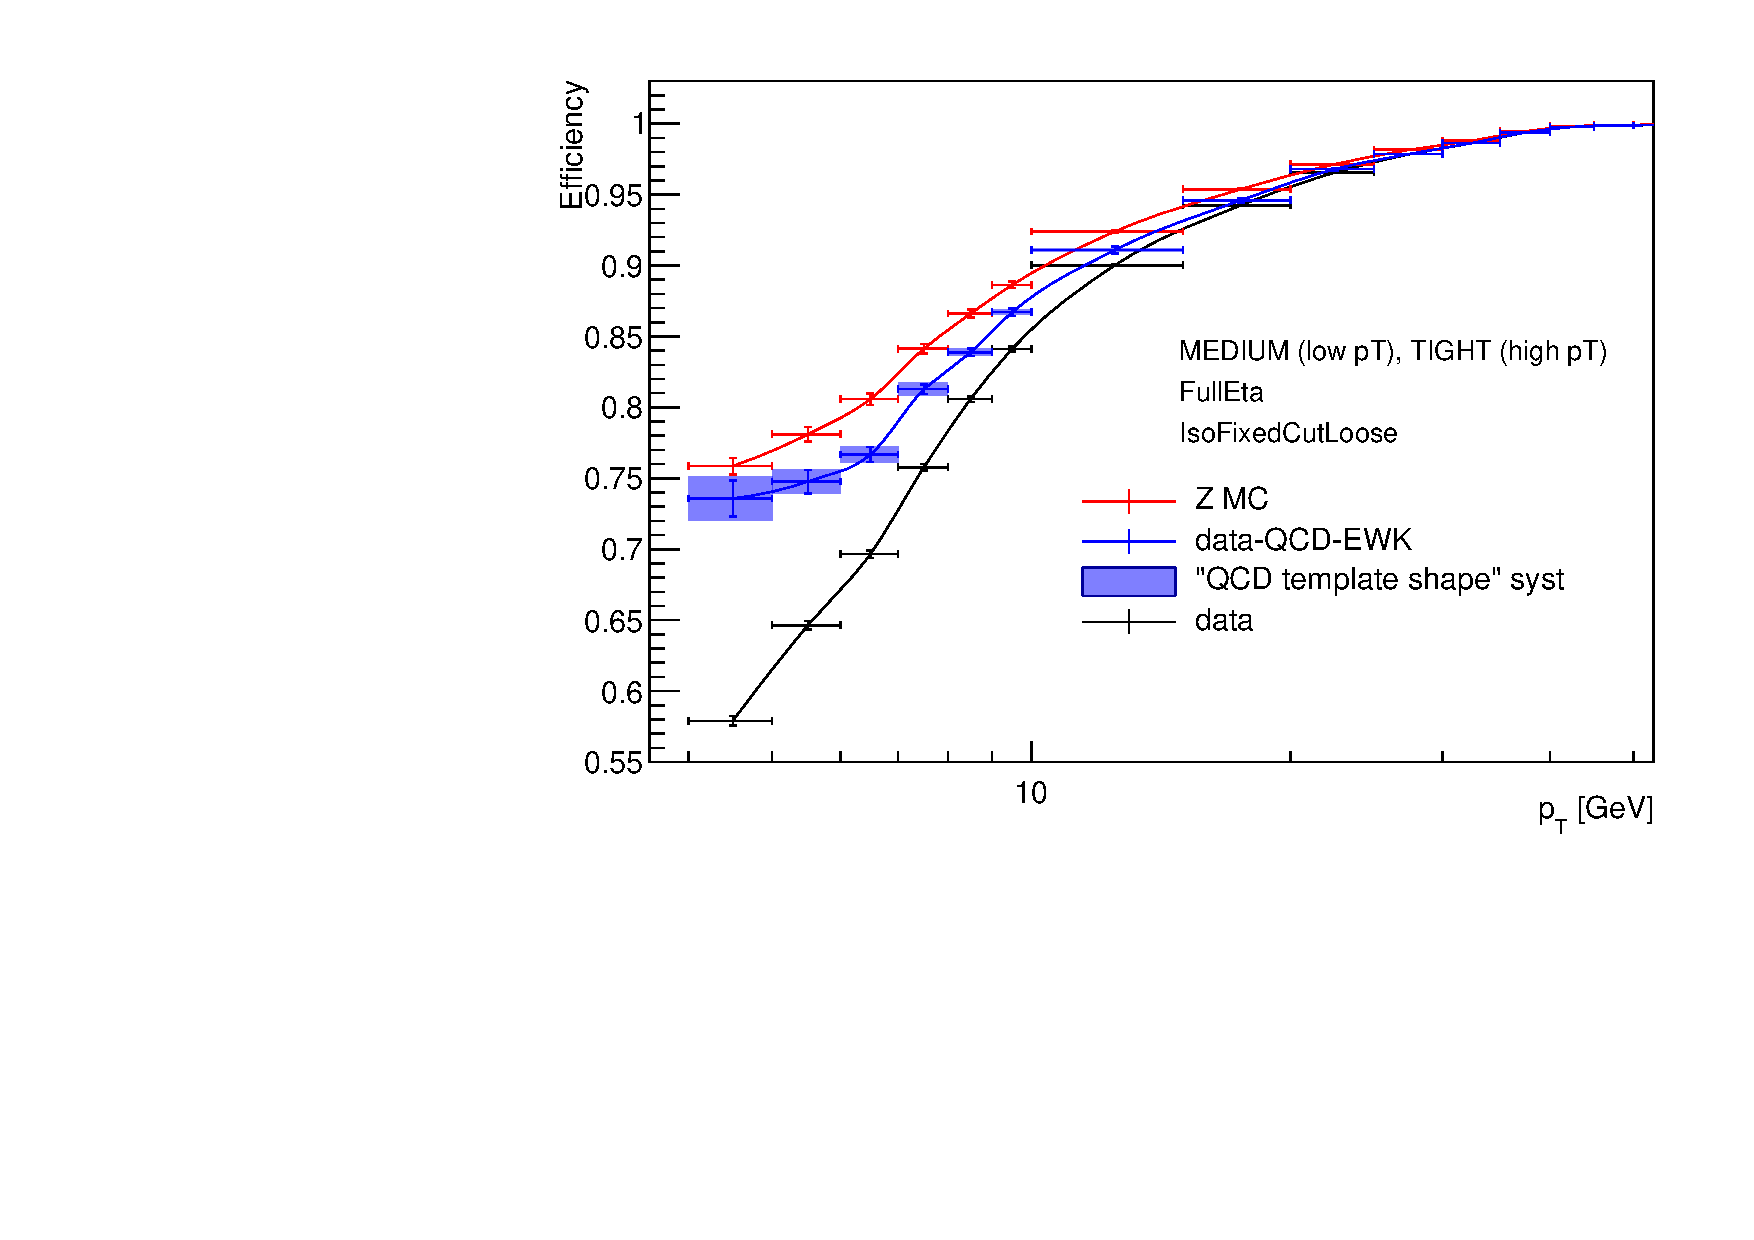
\includegraphics[width=0.8\textwidth]{figures/muons/subtraction}
  \caption[Muon isolation efficiencies.]{Muon isolation efficiencies
  for the FixedCutLoose isolation selection as a function of $\pt$.
  MC simulation efficiency is shown in red, mixed efficiency measured
  in data directly is shown in black, and the $\zmumu$ efficiency
  in data, obtained via the background subtraction, is shown in blue.
  Error bars are statistical, the systematic uncertainty arising from
  the use of different templates is shown as a blue band.}
  \label{fig:muon:sub}
\end{figure}
The efficiencies and scale factors computed with this method, along with
full systematic uncertainties, are shown in Figure \ref{fig:muon:sf} for
the GradientLoose isolation selection.
\begin{figure}[h!]
  \centering
  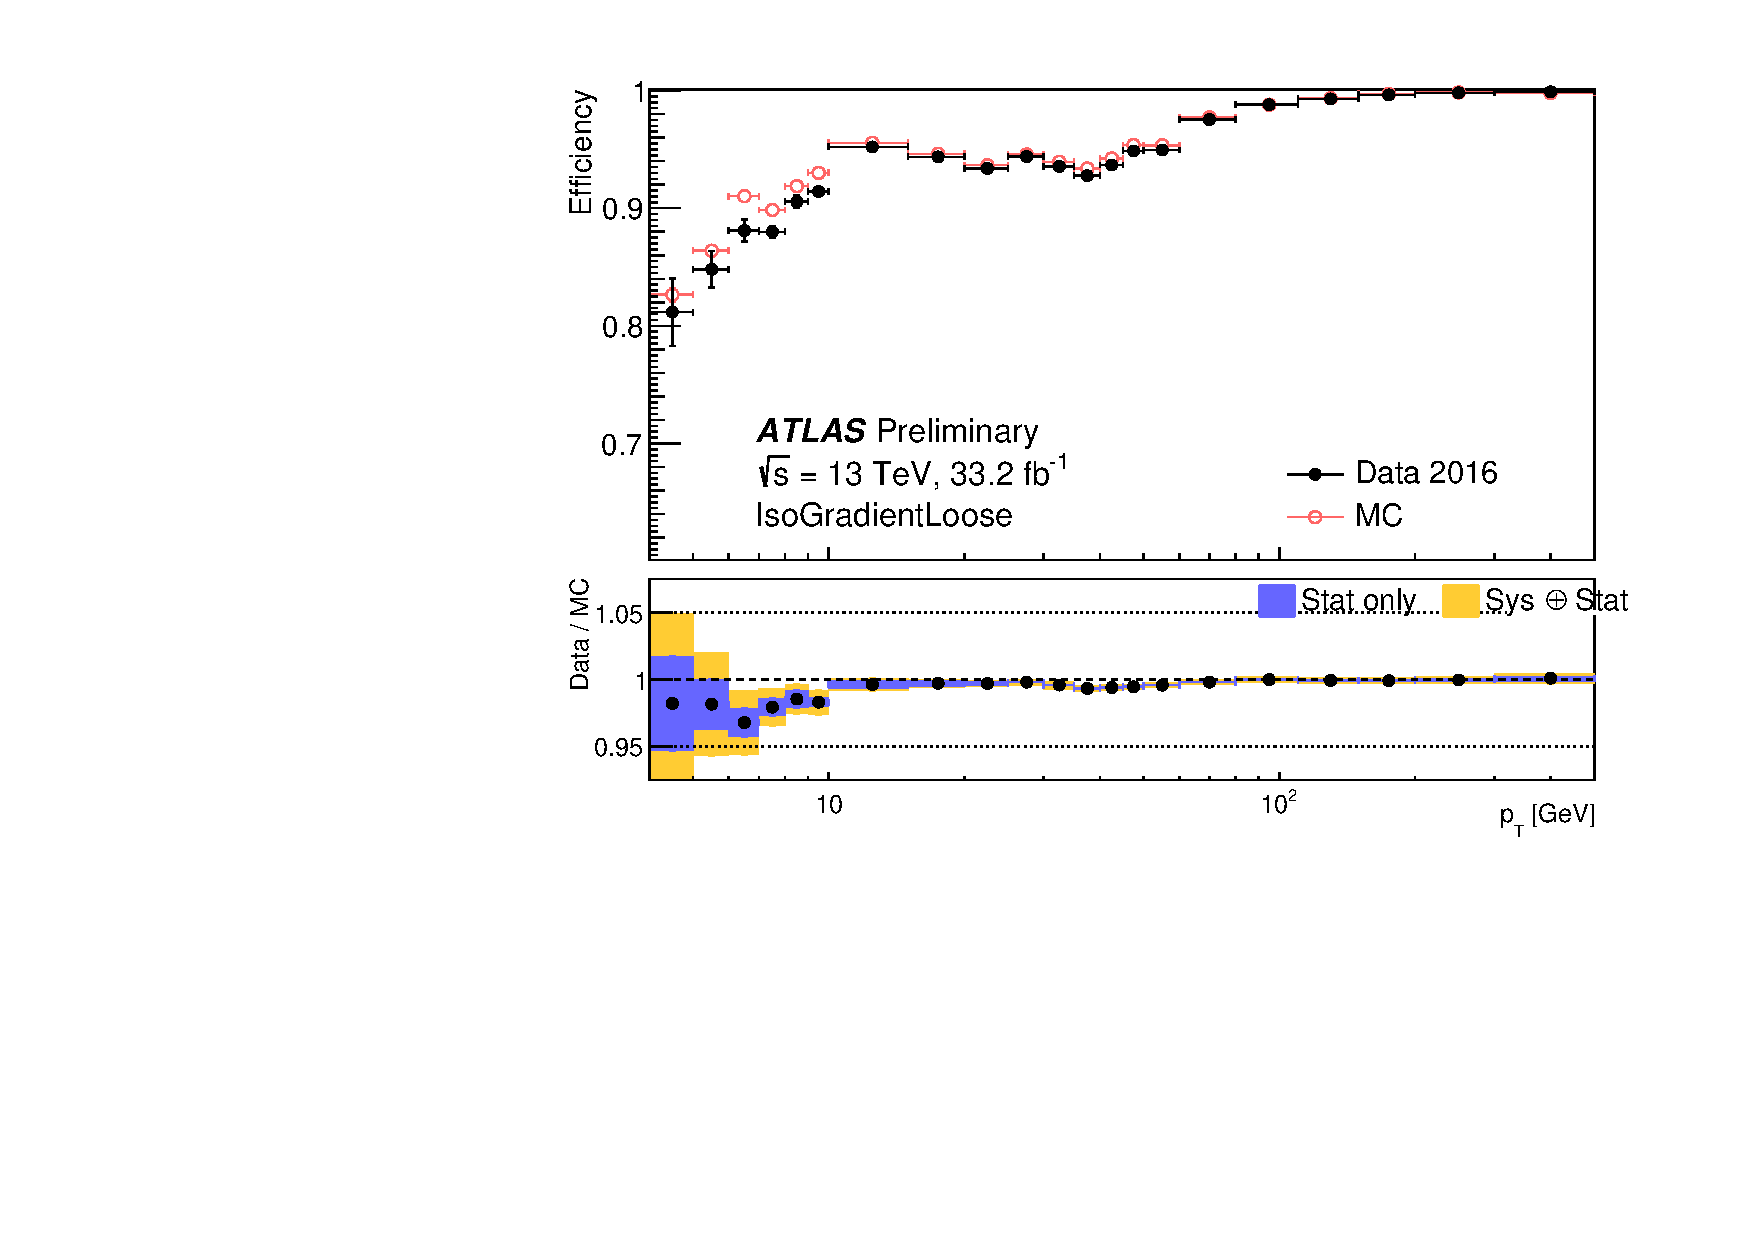
\includegraphics[width=0.8\textwidth]{figures/muons/sf}
  \caption[Muon isolation scale factors.]{Muon isolation efficiencies
  (top panel) and scale factors (bottom panel) for the GradientLoose
  isolation selection as a function of $\pt$ in 2016 data (black filled
  circles) and MC simulation (empty red circles). Error bars represent
  statistical uncertainties, error bands on the scale factors represent
  statistical uncertainties (purple) and statistical and systematic
  uncertainties added in quadrature (yellow).
  From Ref. \cite{Zgubic:2293041}.}
  \label{fig:muon:sf}
\end{figure}
Overall, the method greatly reduces the systematic uncertainty from
background subtraction in the determination of isolation scale factors.
At low $\pt$, where background subtraction used to be the leading
uncertainty, the overall systematic uncertainty on the scale factors
is reduced by up to 75\%. This enabled a better reach in searches for
electroweak SUSY scenarios with compressed mass spectra
\cite{PhysRevD.97.052010} and a more precise studies of low mass
Drell-Yan double differential cross section \cite{Giuli:2681125}.

\section{Other isolation studies}

The muon performance was studied during the collection of 2017 dataset
in order to monitor for any potential problems. No issues were 
found in muon isolation \cite{Bellomo:2282672}.

Furthermore, a few runs in the 2017 dataset were recorded at a particularly high
number of \pileup~interactions, as shown in Figure \ref{fig:exp:pileup}.
These runs were used to perform a study on isolation performance at high
\pileup in preparation for the future runs \cite{Kohler:2293040}.
Figure \ref{fig:muon:highmu} shows the efficiency of the FixedCutTight
selection as a function of muon $\pt$, recorded in 2017 data, separately
for events with more and less than 50 additional interaction vertices
due to \pileup. The  isolation efficiency for the FixedCutTight
selection drops by more than 10\% for muons with $10 < \pt < 20~\GeV$.
\begin{figure}[h!]
  \centering
  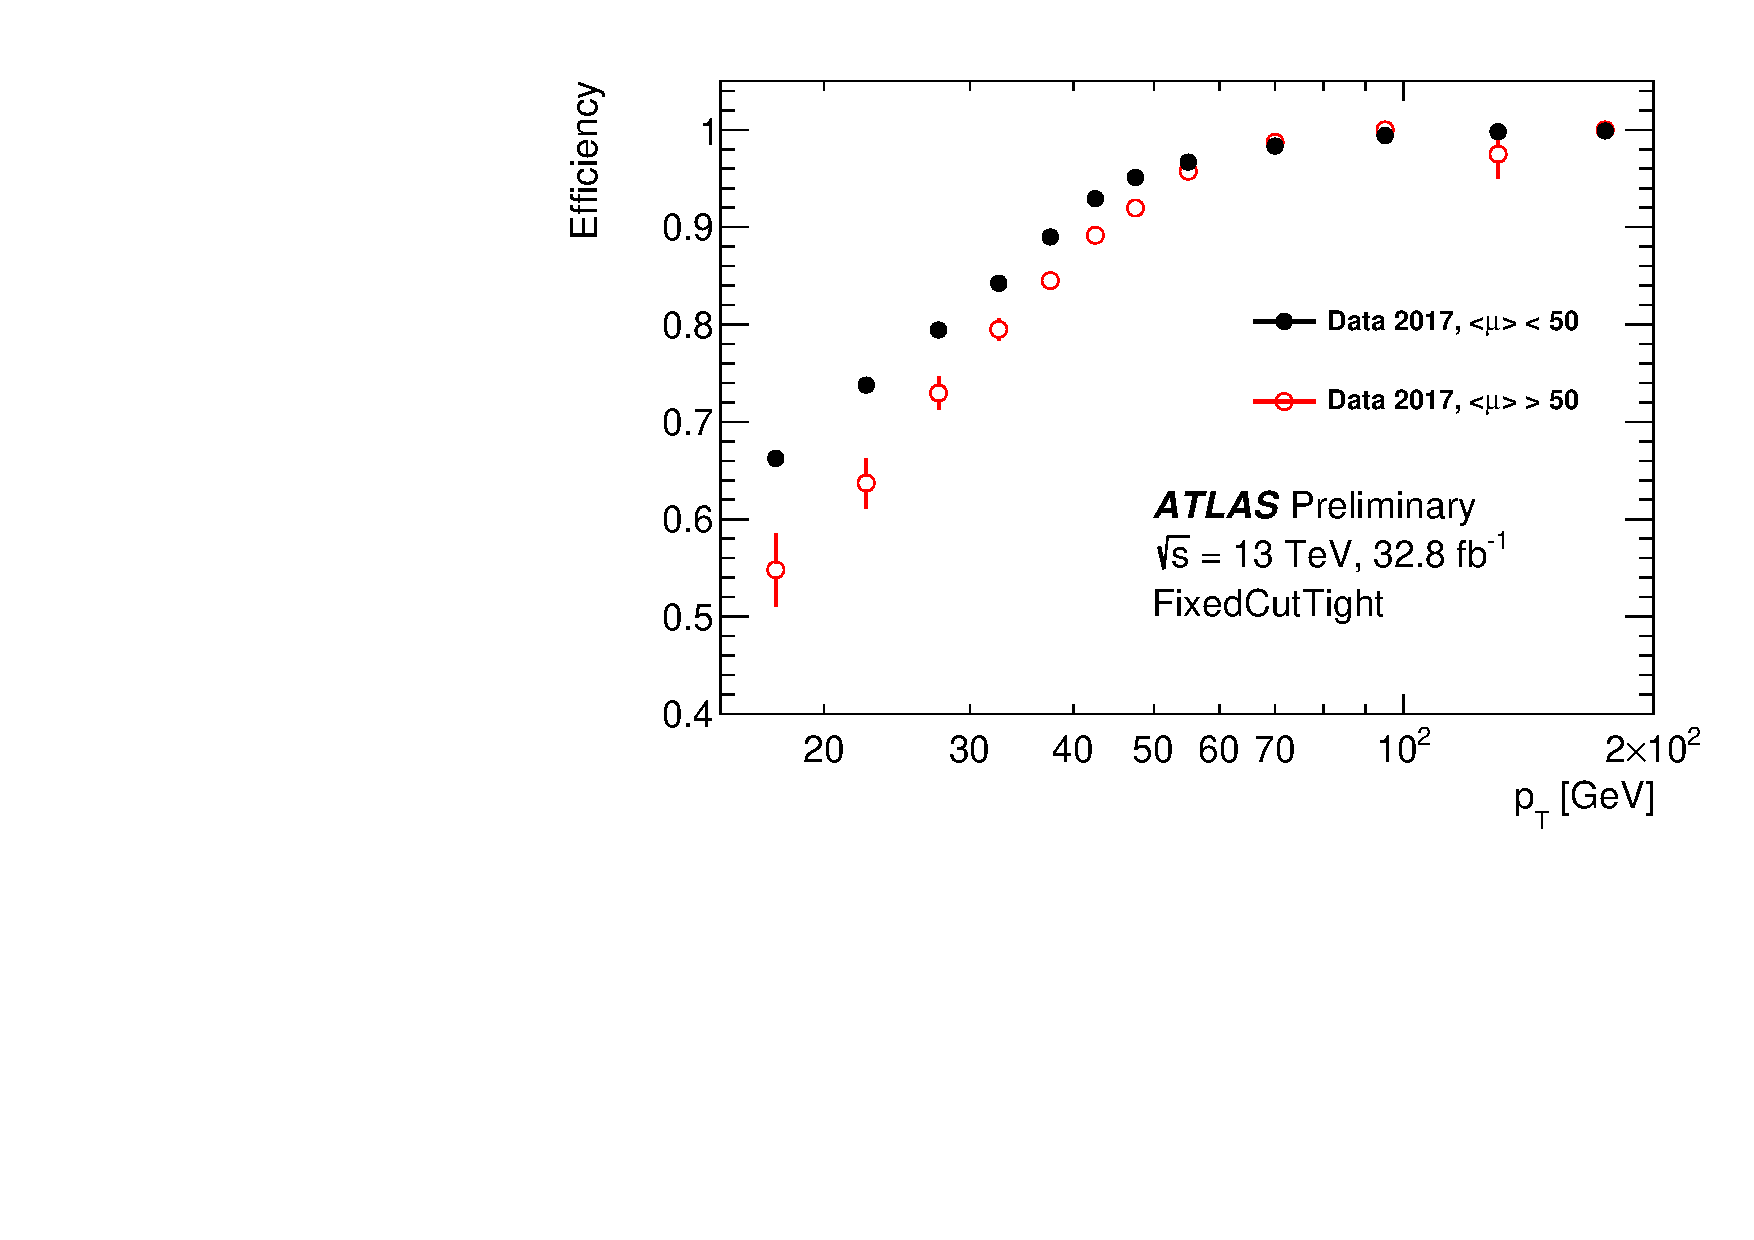
\includegraphics[width=0.8\textwidth]{figures/muons/highmu}
  \caption[Muon isolation efficiency at high \pileup.]{Efficiency
  for the FixedCutTight muon isolation selection as a function of $\pt$
  in 2017 data for events with number of interaction vertices smaller
  than (filled black circles) and larger than (empty red circles) 50.
  No background subtraction is used, and error bars represent
  the statistical uncertainties.
  From Ref. \cite{Kohler:2293040}.}
  \label{fig:muon:highmu}
\end{figure}
This result prompted the development of new isolation selections
designed to be robust against high \pileup~conditions. These new
isolation selections, utilising either a better association of tracks
to the primary interaction vertex (FixedCutHighMuLoose), or by matching
the tracks to clusters in the calorimeters (FixedCutPflowLoose), 
are shown in Figure \ref{fig:muon:newwp} as a function of the number
of \pileup~interactions. The new selections were shown to be more
robust in high \pileup~conditions \cite{Zgubic:2320874}.
\begin{figure}[h!]
  \centering
  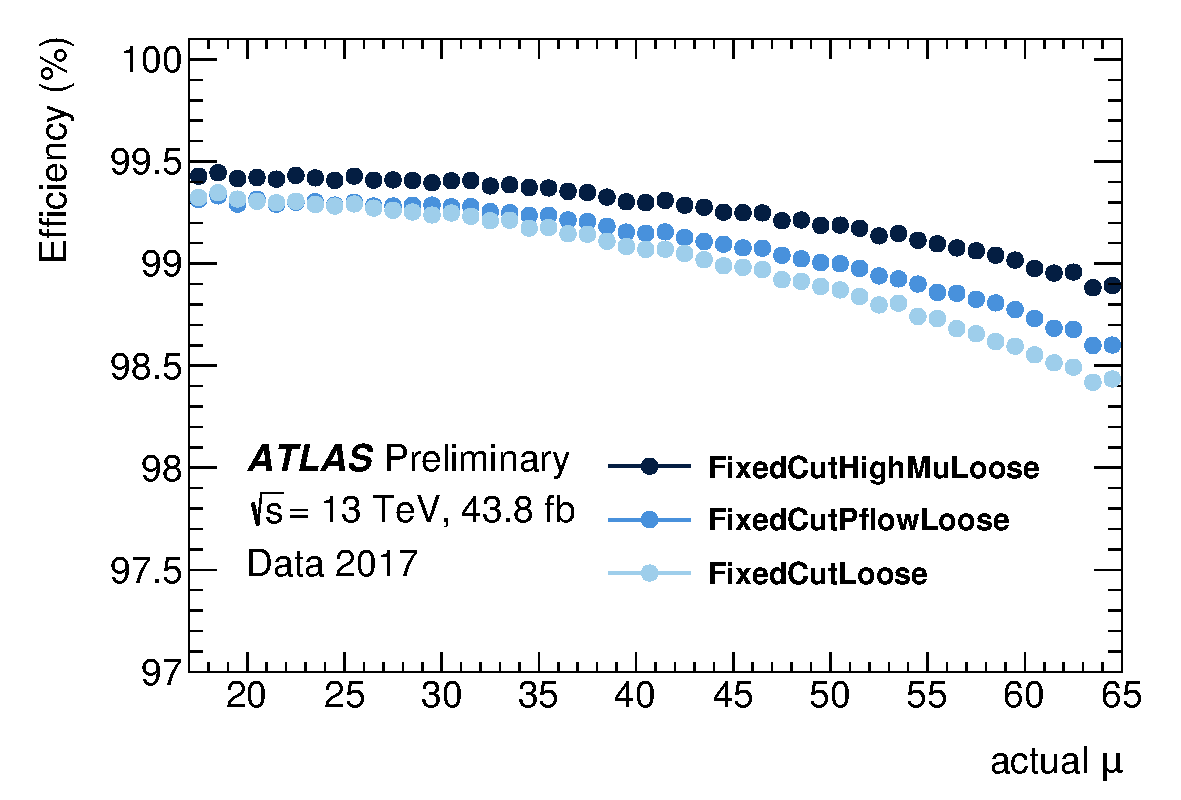
\includegraphics[width=0.8\textwidth]{figures/muons/newwp}
  \caption[Isolation selection robust to high \pileup~conditions.]
  {Efficiency for FixedCutLoose (light blue), FixedCutPflowLoose
  (blue), and FixedCutHighMuLoose (dark blue) isolation selections
  in data collected in 2017 as a function of $\pt$. The errors are
  statistical, and no background subtraction is used.
  From Ref. \cite{Zgubic:2320874}.}
  \label{fig:muon:newwp}
\end{figure}

\section{VADER4$\mu$}

Search for the decay of the Higgs boson to a pair of muons, described
in detail in the next chapter, proceeds as a search for a peak on top
of a smooth Drell-Yan background. According to the Standard Model,
the width of the Higgs boson is much narrower than the experimental
resolution of the ATLAS detector. This could potentially be exploited
the improve the sensitivity of the search and prompted the study to
understand the \textbf{V}ariables \textbf{A}ffecting \textbf{DE}tector
\textbf{R}esolution \textbf{for} \textbf{mu}ons (VADER4$\mu$).

There are two main motivations for the study in the context of
improving the sensitivity of the $\hmumu$ analysis:
\begin{itemize}
\item The muon $\pt$ resolution can be estimated for each individual muon
based on its kinematics and reconstruction quality metrics. The estimated
resolution of individual muons can be propagated to estimate the resolution
of the invariant mass measurement of the muon pair. Finally, the estimate
can be used to split events in resolution categories and the sensitivity of
the analyses may be improved. This can be done directly on the CB muons.
\item Somewhat more speculatively, does the muon reconstruction
algorithms contain bugs, biases, or inefficiencies? Is it possible to 
derive a correction to the muon $\pt$ to improve the dimuon resolution
directly? Ultimately, any potential gain would come from improving the
resolution in data, meaning that the momentum corrections for MC
simulation would have to be re-derived. For this reason, the
corrections would have to be derived separately for the ID and MS
tracks, along with their uncertainties, and combined statistically.
\end{itemize}
Two datasets are prepared to facilitate the study. The "single muon"
dataset consists of reconstructed prompt muons from the MC simulation
of a variety of physics processes, with truth-level $\pt$ information
available. It is preprocessed by removing some of the muons, resulting
in a $\pt$ distribution that is uniform for $\pt < 200~\GeV$. The "dimuon"
dataset consists of data and MC simulation of the $\zmumu$ process
and does not contain any truth-level information. 

Single muon dataset is used to train a gradient boosting regression
model, implemented in \texttt{scikit-learn} \cite{scikit-learn} to
predict the correction to transverse momentum,
$\pt^\text{truth}/\pt^\text{ID}$, from the following variables:
\begin{itemize}
\item $\pt^\text{ID}$, the transverse momentum of the muon as
measured in the ID,
\item $\eta$ and $\phi$ of the muon,
\item $d_0/\sigma_{d_0}$, the transverse impact parameter significance,
\item $z_0$, the longitudinal impact parameter,
\item $\chi^2/N_\text{dof}$, the reduced $\chi^2$ value of the fit,
\item SNS (scattering curvature significance), SCS (scattering
neighbour significance), two variables designed to capture the changes
in track direction across the detector layers in order to detect 
in-flight decays.
\end{itemize}
L1 loss function is used as the L2 loss was found to give biased
results due to asymetric residuals. The equivalent method is used
to predict a correction for the MS muons.

A trained model is then used to provide corrections to the
measured $\pt^\text{ID}$. The distribution of residuals before and
after the correction is shown in Figure \ref{fig:muon:vader-single}
for the training and test splits of the single muon dataset.
The reduction in the standard deviation of the residual distribution
is 17\% for the test set, compared to the uncorrected distribution.
\begin{figure}[h!]
  \centering
  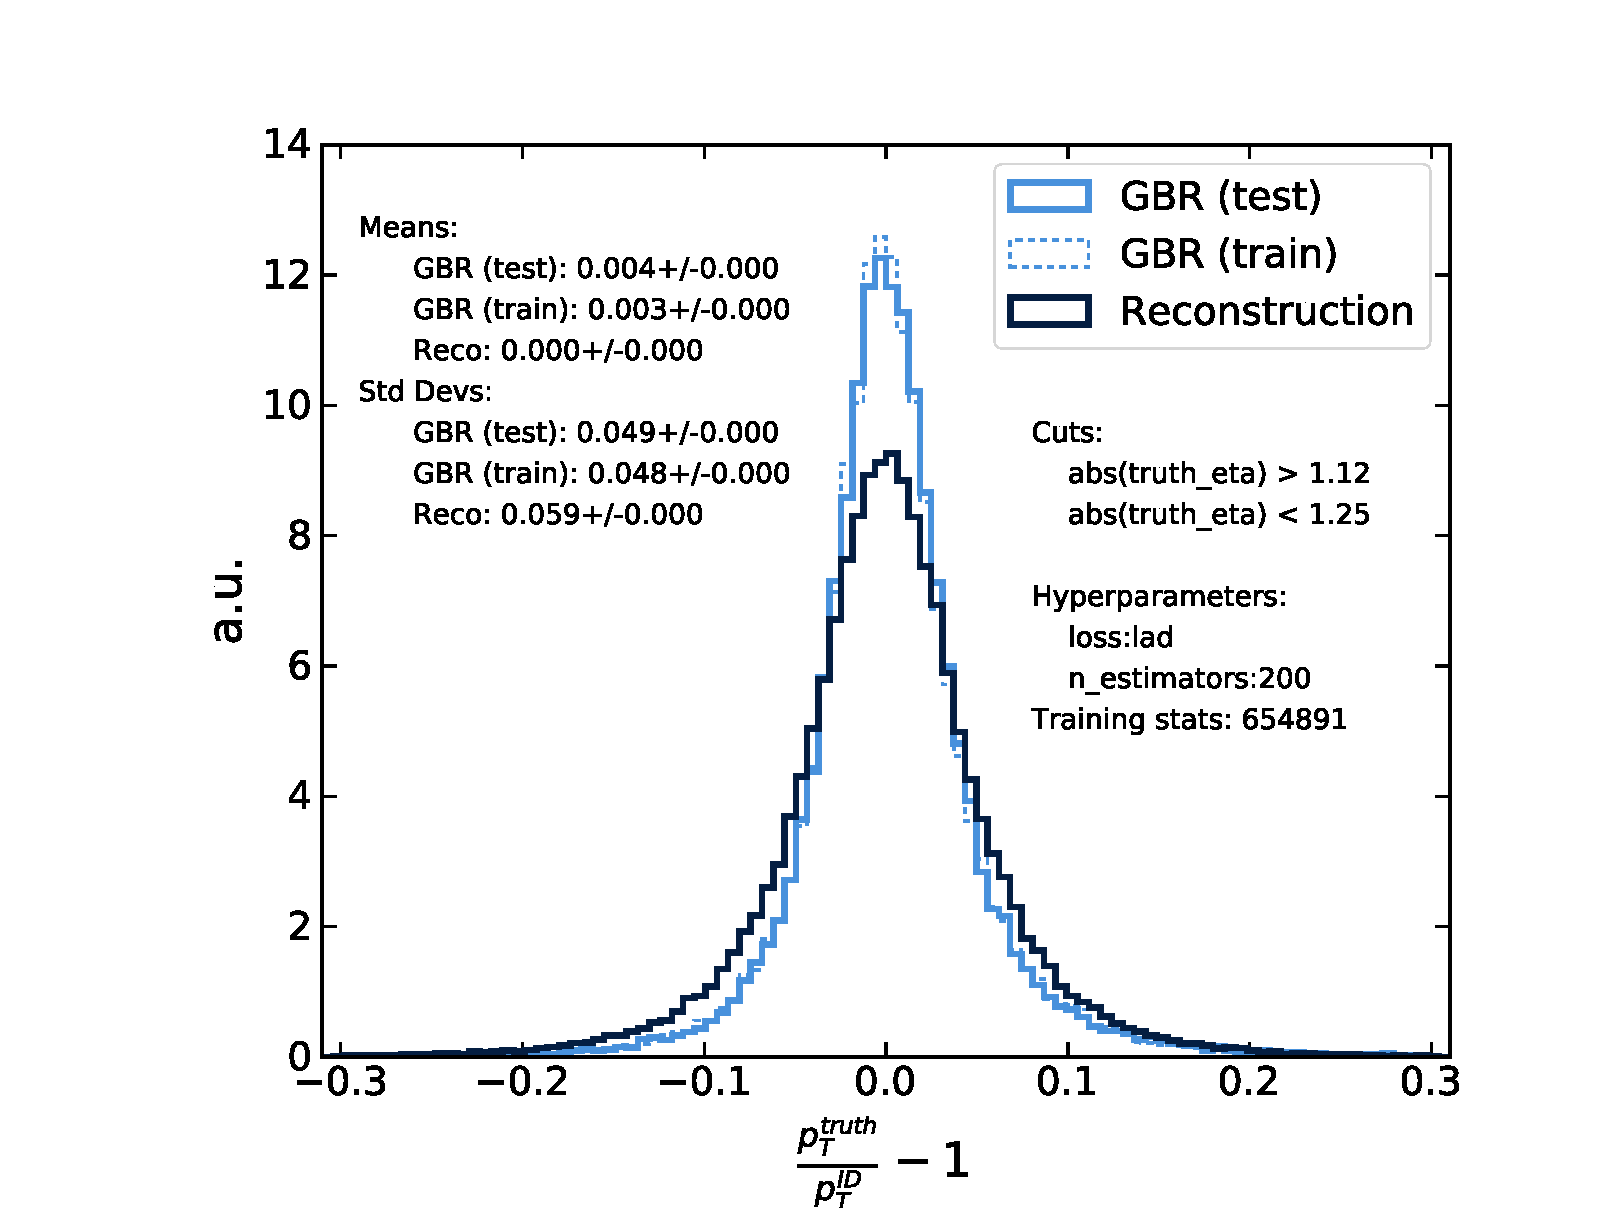
\includegraphics[width=0.8\textwidth]{figures/muons/vader-single}
  \caption[VADER4$\mu$ correction on single muon dataset.]
  {The distribution of residuals for uncorrected (dark blue) and 
  corrected (blue) measurements of momentum for the training (dotted)
  and test (solid) parts of the single muon dataset with
  $1.12 < |\eta| < 1.25$.}
  \label{fig:muon:vader-single}
\end{figure}
A simple grid search, shown in Table \ref{tab:muon:grid} is then
performed to find the best hyperparameter settings. For each 
set of settings in the cartesian product of the search space a
model is trained on the single muon dataset and applied to muons
in the MC simulation part of the dimuon dataset. The full-width
half-maximum of the $Z$ boson peak is chosen as the figure of
merit. The chosen values of the hyperparameters are shown in bold
font in Table \ref{tab:muon:grid}.
\begin{table}[h]
\centering
\caption{VADER4$\mu$ hyperparameter search space with selected settings
in bold text. Other parameters are set to default values.}
\label{tab:muon:grid}
\begin{tabular}{c c c c }
\toprule
Variable & Set of values \\
\midrule
n\_estimators & \{100, 200, 400, \textbf{800}\} \\
max\_depth & \{3, 4, 5, \textbf{6}\} \\
learning\_rate& \{0.001, 0.003, 0.01, \textbf{0.03}, 0.1\} \\
\bottomrule
\end{tabular}
\end{table}
Finally, the 









